\chapter{Projektmanagement}
\label{cha:projekt}
%---------------------------------------- WBS beginnt -----------------------------------------------------------
\section{Work Breakdown Structure}
\label{sec:wbs}

\begin{landscape}
\begin{tikzpicture}[
  basic/.style   = {draw, text width=2.7cm, align=left, drop shadow, rectangle},
  root/.style    = {basic, text width=12cm, rounded corners=2pt, thin, align=center, fill=gray90},
  level 2/.style = {basic, rounded corners=2pt, thin, fill=gray80},
  level 3/.style = {basic, thin, fill=gray90, text width=2.6cm},
  level 1/.style={sibling distance=38mm}, edge from parent fork down, 
  edge from parent/.style={->,draw}, level distance=2.5cm,  >=latex]

% root of the the initial tree, level 1
\node[root] {\tb{Analyse einer ADR-basierten CubeSat-Mission}}
% The first level, as children of the initial tree
  child {node[level 2] (c1) {\tb{AP~1000} \\ Literatur-recherche}}
  child {node[level 2] (c2) {\tb{AP~2000} \\ CubeSat Design}}
  child {node[level 2] (c3) {\tb{AP~3000} \\ Budgetplanung mit QuSad}}
  child {node[level 2] (c4) {\tb{AP~4000} \\ Missions-planung mit GMat}}
  child {node[level 2] (c5) {\tb{AP~5000} \\ Dokumentation \\ $~~$}};

% The second level, relatively positioned nodes
\begin{scope}[every node/.style={level 3}, node distance=6pt]
\node [below=of c1, xshift=10pt] (c11) {\tb{AP~1100} \\ Weltraumm\"ull-problematik};
\node [below=of c11] (c12) {\tb{AP~1200} \\ CubeSat Subsysteme};
\node [below=of c12] (c13) {\tb{AP~1300} \\ Rendezvou und Docking};
\node [below=of c13] (c14) {\tb{AP~1400} \\ Erforderliche Softwares};


\node [below=of c2, xshift=10pt] (c21) {\tb{AP~2100} \\ CubeSat Datenbank Analyse};
\node [below=of c21] (c22) {\tb{AP~2200} \\ Ausarbeitung von Subsystemen};
\node [below=of c22] (c23) {\tb{AP~2300} \\ Ausarbeitung von CubeSat Konfigurationen};

\node [below=of c3, xshift=10pt] (c31) {\tb{AP~3100} \\ Datenbank-erweiterung};
\node [below=of c31] (c32) {\tb{AP~3200} \\ Generierung der CubeSat Konfigurationen};
\node [below=of c32] (c33) {\tb{AP~3300} \\ Budget-kalkulation und Vergleich};

\node [below=of c4, xshift=10pt] (c41) {\tb{AP~4100} \\ Missions-auslegung};
\node [below=of c41] (c42) {\tb{AP~4200} \\ Durchführung der Simulation};
\node [below=of c42] (c43) {\tb{AP~4300} \\ Auswertung der Simulation};

\node [below=of c5, xshift=10pt] (c51) {\tb{AP~5100} \\ Textverfassung};
\node [below=of c51] (c52) {\tb{AP~5200} \\ Überprüfung};

\end{scope}
%--------------------------------------------- Pfeile für das Diagramm vom WBS -------------------------------------
%-----------------------------------lines from each level 1 node to every one of its "children"--------------------
\foreach \value in {1,2,3,4}
  \draw[->] (c1.212) |- (c1\value.west);

\foreach \value in {1,2,3}
  \draw[->] (c2.212) |- (c2\value.west);

\foreach \value in {1,2,3}
  \draw[->] (c3.212) |- (c3\value.west);

\foreach \value in {1,2,3}
  \draw[->] (c4.212) |- (c4\value.west);

\foreach \value in {1,2}
  \draw[->] (c5.212) |- (c5\value.west);
  
\end{tikzpicture}
\end{landscape}

\section{Zeitplan}
%----------------------------------------------- Ganttchart Diagramm -----------------------------------------------
	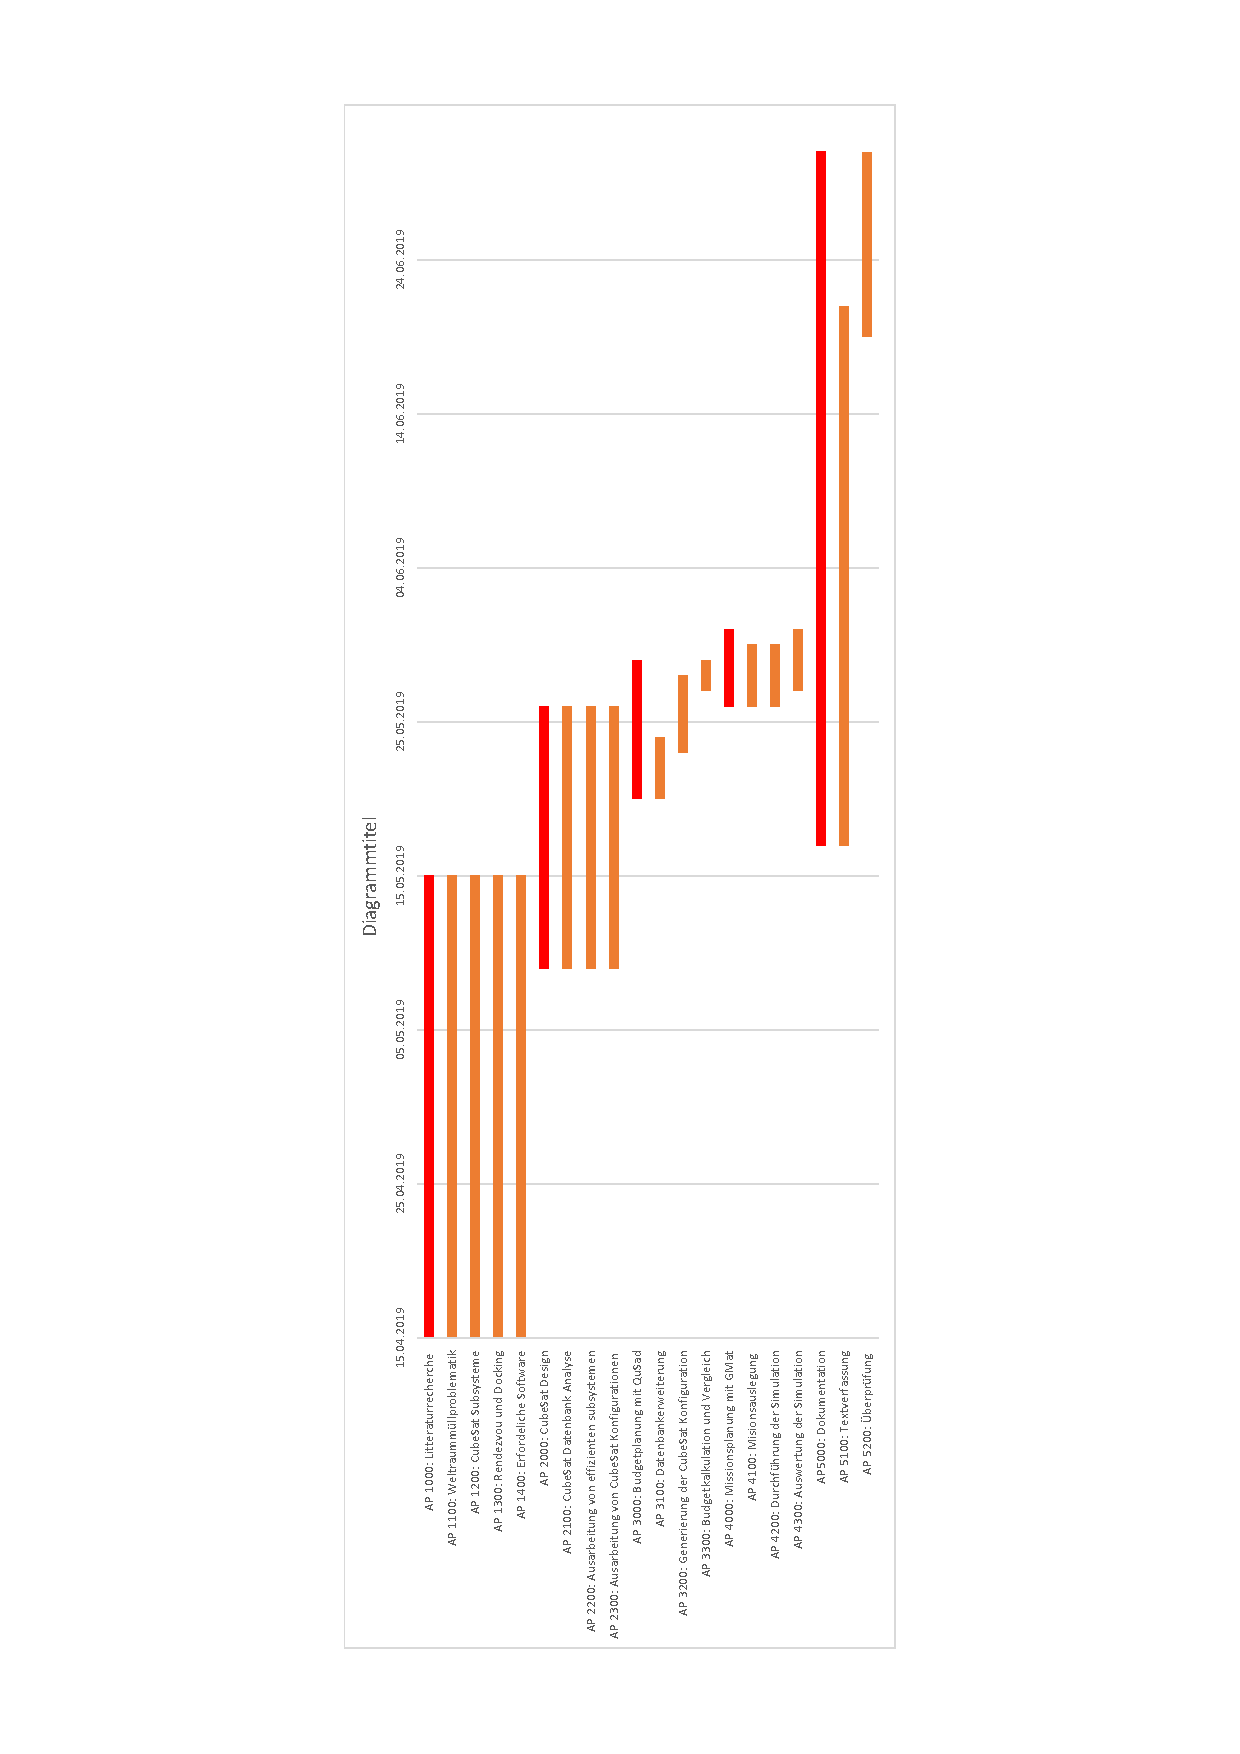
\includepdf[pages=-]{./pdf/Mappe1.pdf}			%PDF-Datei wird hinzugefügt Ganttchart

\section{Work Package Description}
\label{sec:wpd}


%--------------------------------------------- AP Literaturrecherche ------------------------------------------
%-------------------------------------------- Tabelle Weltraummüllproblematik ---------------------------------
\begin{table}[!h]
 \begin{center}
  \begin{tabular}{|p{35mm}||p{55mm}|p{50mm}||p{40mm}|}
   \hline
   \multicolumn{3}{|l||}{\textbf{}} & \multicolumn{1}{c|}{}\\
   \multicolumn{3}{|l||}{\textbf{}} & \multicolumn{1}{c|}{\textbf{AP 1100}}\\
   \multicolumn{3}{|l||}{\textbf{}} & \multicolumn{1}{c|}{}\\
   \hline\hline
   \textbf{Titel} & \multicolumn{2}{p{7cm}||}{\textbf{Weltraummüllproblematik}} & \textbf{Seite:} 1 von 1\\
   \hline
   \textbf{Verantwortlicher} & \multicolumn{2}{l||}{Frederik Schäfer} & \textbf{Version:} 1.1\\
   \hline
   \multicolumn{3}{|l||}{} & \textbf{Datum:} 15.04.2019\\
   \hline\hline
   \textbf{Beginn} & \multicolumn{2}{l||}{15.04.2019} & \\
   \hline
   \textbf{Ende} & \multicolumn{2}{l||}{15.05.2019} & \textbf{Dauer}: 30 Tage\\
   \hline\hline
   \textbf{Bearbeiter} & \multicolumn{3}{l|}{F. Czorny, F. Schäfer, M. Strempel, O. Mouhaya, V. Dietrich}\\
   \hline\hline
   \multicolumn{4}{|p{150mm}|}{\textbf{Ziele:}}\\
   \multicolumn{4}{|p{150mm}|}{$\bullet$ Verstehen von Weltraummüll Entwicklung}\\
   \multicolumn{4}{|p{150mm}|}{$\bullet$ Verstehen der resultierenden Risiken}\\
   \multicolumn{4}{|p{150mm}|}{}\\
   \multicolumn{4}{|p{150mm}|}{\textbf{Input:}}\\
   \multicolumn{4}{|p{150mm}|}{$\bullet$ Literatur zu Weltraummüll und Megakonstellationen}\\
   \multicolumn{4}{|p{150mm}|}{}\\
   \multicolumn{4}{|p{150mm}|}{\textbf{Aufgaben:}}\\
   \multicolumn{4}{|p{150mm}|}{$\bullet$ Literatur sichten}\\
   \multicolumn{4}{|p{150mm}|}{$\bullet$ Ziele des Projekts definieren}\\
   \multicolumn{4}{|p{150mm}|}{}\\
   \hline
  \end{tabular}
 \end{center}
\end{table}

\clearpage
%-------------------------------------------- Tabelle CubeSat Subsysteme ----------------------------------------
\begin{table}[!h]
 \begin{center}
  \begin{tabular}{|p{35mm}||p{55mm}|p{50mm}||p{40mm}|}
   \hline
   \multicolumn{3}{|l||}{\textbf{}} & \multicolumn{1}{c|}{}\\
   \multicolumn{3}{|l||}{\textbf{}} & \multicolumn{1}{c|}{\textbf{AP 1200}}\\
   \multicolumn{3}{|l||}{\textbf{}} & \multicolumn{1}{c|}{}\\
   \hline\hline
   \textbf{Titel} & \multicolumn{2}{p{7cm}||}{\textbf{CubeSat Subsysteme}} & \textbf{Seite:} 1 von 1\\
   \hline
   \textbf{Verantwortlicher} & \multicolumn{2}{l||}{Frederik Schäfer} & \textbf{Version:} 1.1\\
   \hline
   \multicolumn{3}{|l||}{} & \textbf{Datum:} 15.04.2019\\
   \hline\hline
   \textbf{Beginn} & \multicolumn{2}{l||}{15.04.2019} & \\
   \hline
   \textbf{Ende} & \multicolumn{2}{l||}{15.05.2019} & \textbf{Dauer}: 30 Tage\\
   \hline\hline
   \textbf{Bearbeiter} & \multicolumn{3}{l|}{F. Czorny, F. Schäfer, M. Strempel, O. Mouhaya, V. Dietrich}\\
   \hline\hline
   \multicolumn{4}{|p{150mm}|}{\textbf{Ziele:}}\\
   \multicolumn{4}{|p{150mm}|}{$\bullet$ Kennenlernen und Verstehen der CubeSat Subsysteme}\\
   \multicolumn{4}{|p{150mm}|}{}\\
   \multicolumn{4}{|p{150mm}|}{\textbf{Input:}}\\
   \multicolumn{4}{|p{150mm}|}{$\bullet$ Literatur zu CubeSat Subsystemen}\\
   \multicolumn{4}{|p{150mm}|}{}\\
   \multicolumn{4}{|p{150mm}|}{\textbf{Aufgaben:}}\\
   \multicolumn{4}{|p{150mm}|}{$\bullet$ Literatur sichten}\\
   \multicolumn{4}{|p{150mm}|}{$\bullet$ Informationen über Subsysteme zusammenfassen}\\
   \multicolumn{4}{|p{150mm}|}{}\\
   \hline
  \end{tabular}
 \end{center}
\end{table}

\clearpage
%-------------------------------------------- Tabelle Rendezvous und Docking -------------------------------
\begin{table}[!h]
 \begin{center}
  \begin{tabular}{|p{35mm}||p{55mm}|p{50mm}||p{40mm}|}
   \hline
   \multicolumn{3}{|l||}{\textbf{}} & \multicolumn{1}{c|}{}\\
   \multicolumn{3}{|l||}{\textbf{}} & \multicolumn{1}{c|}{\textbf{AP 1300}}\\
   \multicolumn{3}{|l||}{\textbf{}} & \multicolumn{1}{c|}{}\\
   \hline\hline
   \textbf{Titel} & \multicolumn{2}{p{7cm}||}{\textbf{Rendezvous und Docking}} & \textbf{Seite:} 1 von 1\\
   \hline
   \textbf{Verantwortlicher} & \multicolumn{2}{l||}{Frederik Schäfer} & \textbf{Version:} 1.1\\
   \hline
   \multicolumn{3}{|l||}{} & \textbf{Datum:} 15.04.2019\\
   \hline\hline
   \textbf{Beginn} & \multicolumn{2}{l||}{15.04.2019} & \\
   \hline
   \textbf{Ende} & \multicolumn{2}{l||}{15.05.2019} & \textbf{Dauer}: 30 Tage\\
   \hline\hline
   \textbf{Bearbeiter} & \multicolumn{3}{l|}{F. Czorny, F. Schäfer, M. Strempel, O. Mouhaya, V. Dietrich}\\
   \hline\hline
   \multicolumn{4}{|p{150mm}|}{\textbf{Ziele:}}\\
   \multicolumn{4}{|p{150mm}|}{$\bullet$ Kennenlernen und Verstehen von RDV und Docking Vorgängen mit nichtkooperativen Zielen}\\
   \multicolumn{4}{|p{150mm}|}{}\\
   \multicolumn{4}{|p{150mm}|}{\textbf{Input:}}\\
   \multicolumn{4}{|p{150mm}|}{$\bullet$ Literatur zu RDV und Docking mit nichtkooperativen Zielen}\\
   \multicolumn{4}{|p{150mm}|}{}\\
   \multicolumn{4}{|p{150mm}|}{\textbf{Schnittstellen zu anderen APs:}}\\
   \multicolumn{4}{|p{150mm}|}{$\bullet$ \textbf{AP 1200} für Verständnis der notwendigen Subsysteme}\\
   \multicolumn{4}{|p{150mm}|}{$\bullet$ \textbf{AP 1100} für Verständnis von Zielteilen}\\
   \multicolumn{4}{|p{150mm}|}{}\\
   \multicolumn{4}{|p{150mm}|}{\textbf{Aufgaben:}}\\
   \multicolumn{4}{|p{150mm}|}{$\bullet$ Literatur sichten}\\
   \multicolumn{4}{|p{150mm}|}{}\\
   \hline
  \end{tabular}
 \end{center}
\end{table}

\clearpage
%-------------------------------------------- Tabelle Erforderliche Software ------------------------------
\begin{table}[!h]
 \begin{center}
  \begin{tabular}{|p{35mm}||p{55mm}|p{50mm}||p{40mm}|}
   \hline
   \multicolumn{3}{|l||}{\textbf{}} & \multicolumn{1}{c|}{}\\
   \multicolumn{3}{|l||}{\textbf{}} & \multicolumn{1}{c|}{\textbf{AP 1400}}\\
   \multicolumn{3}{|l||}{\textbf{}} & \multicolumn{1}{c|}{}\\
   \hline\hline
   \textbf{Titel} & \multicolumn{2}{p{7cm}||}{\textbf{Software}} & \textbf{Seite:} 1 von 1\\
   \hline
   \textbf{Verantwortlicher} & \multicolumn{2}{l||}{Frederik Schäfer} & \textbf{Version:} 1.1\\
   \hline
   \multicolumn{3}{|l||}{} & \textbf{Datum:} 15.04.2019\\
   \hline\hline
   \textbf{Beginn} & \multicolumn{2}{l||}{15.04.2019} & \\
   \hline
   \textbf{Ende} & \multicolumn{2}{l||}{15.05.2019} & \textbf{Dauer}: 30 Tage\\
   \hline\hline
   \textbf{Bearbeiter} & \multicolumn{3}{l|}{F. Czorny, F. Schäfer, M. Strempel, O. Mouhaya, V. Dietrich}\\
   \hline\hline
   \multicolumn{4}{|p{150mm}|}{\textbf{Ziele:}}\\
   \multicolumn{4}{|p{150mm}|}{$\bullet$ Software ist Einsatzbereit}\\
   \multicolumn{4}{|p{150mm}|}{}\\
   \multicolumn{4}{|p{150mm}|}{\textbf{Input:}}\\
   \multicolumn{4}{|p{150mm}|}{$\bullet$ QuSAD, GMAT, LaTeX}\\
   \multicolumn{4}{|p{150mm}|}{$\bullet$ MatLab, Citavi, GitHub}\\
   \multicolumn{4}{|p{150mm}|}{}\\
   \multicolumn{4}{|p{150mm}|}{\textbf{Aufgaben:}}\\
   \multicolumn{4}{|p{150mm}|}{$\bullet$ Installieren der Software}\\
   \multicolumn{4}{|p{150mm}|}{$\bullet$ Einarbeitung in Programme}\\
   \multicolumn{4}{|p{150mm}|}{}\\
   \hline
  \end{tabular}
 \end{center}
\end{table}

\clearpage
%-------------------------------------------- AP Cubesat Design -----------------------------------------------
%------------------------------------ Tabelle CubeSat Datenbank Analyse ---------------------------------------
\begin{table}[!h]
 \begin{center}
  \begin{tabular}{|p{35mm}||p{55mm}|p{50mm}||p{40mm}|}
   \hline
   \multicolumn{3}{|l||}{\textbf{}} & \multicolumn{1}{c|}{}\\
   \multicolumn{3}{|l||}{\textbf{}} & \multicolumn{1}{c|}{\textbf{AP 2100}}\\
   \multicolumn{3}{|l||}{\textbf{}} & \multicolumn{1}{c|}{}\\
   \hline\hline
   \textbf{Titel} & \multicolumn{2}{p{7cm}||}{\textbf{CubeSat Datenbank Analyse}} & \textbf{Seite:} 1 von 1\\
   \hline
   \textbf{Verantwortlicher} & \multicolumn{2}{l||}{Florian Czorny} & \textbf{Version:} 1.1\\
   \hline
   \multicolumn{3}{|l||}{} & \textbf{Datum:} 15.04.2019\\
   \hline\hline
   \textbf{Beginn} & \multicolumn{2}{l||}{09.05.2019} & \\
   \hline
   \textbf{Ende} & \multicolumn{2}{l||}{26.05.2019} & \textbf{Dauer}: 17 Tage\\
   \hline\hline
   \textbf{Bearbeiter} & \multicolumn{3}{l|}{V. Dietrich, F. Czorny}\\
   \hline\hline
   \multicolumn{4}{|p{150mm}|}{\textbf{Ziele:}}\\
   \multicolumn{4}{|p{150mm}|}{$\bullet$ Auseinandersetzung mit der Datenbank }\\
   \multicolumn{4}{|p{150mm}|}{}\\
   \multicolumn{4}{|p{150mm}|}{\textbf{Schnittstellen zu anderen APs:}}\\
   \multicolumn{4}{|p{150mm}|}{$\bullet$ \textbf{AP 2200} Überblick über vorhandene Subsysteme }\\
   \multicolumn{4}{|p{150mm}|}{$\bullet$ \textbf{AP 2300} Überblick über vorhandene Subsysteme }\\
	 \multicolumn{4}{|p{150mm}|}{$\bullet$ \textbf{AP 3100} Ermitteln fehlender Daten}\\
   \multicolumn{4}{|p{150mm}|}{}\\
   \multicolumn{4}{|p{150mm}|}{\textbf{Aufgaben:}}\\
   \multicolumn{4}{|p{150mm}|}{$\bullet$ Kenntnisse über Inhalt der Datenbank erlangen}\\
   \multicolumn{4}{|p{150mm}|}{$\bullet$ Überblick über vorhandene Subsysteme erlangen}\\
   \multicolumn{4}{|p{150mm}|}{}\\
   \hline
  \end{tabular}
 \end{center}
\end{table}

\clearpage
%------------------------------------ Tabelle Ausarbeitung von effizienten Subsystemen -------------------------------------
\begin{table}[!h]
 \begin{center}
  \begin{tabular}{|p{35mm}||p{55mm}|p{50mm}||p{40mm}|}
   \hline
   \multicolumn{3}{|l||}{\textbf{}} & \multicolumn{1}{c|}{}\\
   \multicolumn{3}{|l||}{\textbf{}} & \multicolumn{1}{c|}{\textbf{AP 2200}}\\
   \multicolumn{3}{|l||}{\textbf{}} & \multicolumn{1}{c|}{}\\
   \hline\hline
   \textbf{Titel} & \multicolumn{2}{p{7cm}||}{\textbf{Ausarbeitung von Subsystemen}} & \textbf{Seite:} 1 von 1\\
   \hline
   \textbf{Verantwortlicher} & \multicolumn{2}{l||}{Florian Czorny} & \textbf{Version:} 1.1\\
   \hline
   \multicolumn{3}{|l||}{} & \textbf{Datum:} 15.04.2019\\
   \hline\hline
   \textbf{Beginn} & \multicolumn{2}{l||}{09.05.2019} & \\
   \hline
   \textbf{Ende} & \multicolumn{2}{l||}{26.05.2019} & \textbf{Dauer}: 17 Tage\\
   \hline\hline
   \textbf{Bearbeiter} & \multicolumn{3}{l|}{V. Dietrich, F. Czorny}\\
   \hline\hline
   \multicolumn{4}{|p{150mm}|}{\textbf{Ziele:}}\\
   \multicolumn{4}{|p{150mm}|}{$\bullet$ Auswahl qualifizierter Subsysteme}\\
   \multicolumn{4}{|p{150mm}|}{}\\
   \multicolumn{4}{|p{150mm}|}{\textbf{Input:}}\\
   \multicolumn{4}{|p{150mm}|}{$\bullet$ \textbf{AP 2100} Vorhandene Subsysteme in der Datenbank}\\
   \multicolumn{4}{|p{150mm}|}{}\\
   \multicolumn{4}{|p{150mm}|}{\textbf{Schnittstellen zu anderen APs:}}\\
   \multicolumn{4}{|p{150mm}|}{$\bullet$ \textbf{AP 2300} Vorauswahl für die Konfigurationen}\\
   \multicolumn{4}{|p{150mm}|}{}\\
   \multicolumn{4}{|p{150mm}|}{\textbf{Aufgaben:}}\\
   \multicolumn{4}{|p{150mm}|}{$\bullet$ Verwendbare Subsysteme identifizieren und vergleichen}\\
   \multicolumn{4}{|p{150mm}|}{}\\
   \hline
  \end{tabular}
 \end{center}
\end{table}

\clearpage
%----------------------------------- Tabelle Ausarbeitung von CubeSat Konfigurationen ----------------------------------------
\begin{table}[!h]
 \begin{center}
  \begin{tabular}{|p{35mm}||p{55mm}|p{50mm}||p{40mm}|}
   \hline
   \multicolumn{3}{|l||}{\textbf{}} & \multicolumn{1}{c|}{}\\
   \multicolumn{3}{|l||}{\textbf{}} & \multicolumn{1}{c|}{\textbf{AP 2300}}\\
   \multicolumn{3}{|l||}{\textbf{}} & \multicolumn{1}{c|}{}\\
   \hline\hline
   \textbf{Titel} & \multicolumn{2}{p{7cm}||}{\textbf{Ausarbeitung von CubeSat Konfigurationen}} & \textbf{Seite:} 1 von 1\\
   \hline
   \textbf{Verantwortlicher} & \multicolumn{2}{l||}{Florian Czorny} & \textbf{Version:} 1.1\\
   \hline
   \multicolumn{3}{|l||}{} & \textbf{Datum:} 15.04.2019\\
   \hline\hline
   \textbf{Beginn} & \multicolumn{2}{l||}{09.05.2019} & \\
   \hline
   \textbf{Ende} & \multicolumn{2}{l||}{26.05.2019} & \textbf{Dauer}: 17 Tage\\
   \hline\hline
   \textbf{Bearbeiter} & \multicolumn{3}{l|}{V. Dietrich, F. Czorny}\\
   \hline\hline
   \multicolumn{4}{|p{150mm}|}{\textbf{Ziele:}}\\
   \multicolumn{4}{|p{150mm}|}{$\bullet$ Zusammenstellung ausgewählter Konfigurationen}\\
   \multicolumn{4}{|p{150mm}|}{}\\
   \multicolumn{4}{|p{150mm}|}{\textbf{Input:}}\\
   \multicolumn{4}{|p{150mm}|}{$\bullet$ \textbf{AP 2200} Vorauswahl der Subsysteme}\\
   \multicolumn{4}{|p{150mm}|}{}\\
   \multicolumn{4}{|p{150mm}|}{\textbf{Schnittstellen zu anderen APs:}}\\
   \multicolumn{4}{|p{150mm}|}{$\bullet$ \textbf{AP 3100} Möglicherweise nicht alle Komponenten in der Datenbank}\\
   \multicolumn{4}{|p{150mm}|}{$\bullet$ \textbf{AP 3200} verfeinert erfasste Konfigurationen}\\
   \multicolumn{4}{|p{150mm}|}{}\\
   \multicolumn{4}{|p{150mm}|}{\textbf{Aufgaben:}}\\
   \multicolumn{4}{|p{150mm}|}{$\bullet$ Verschiedene Konfigurationen der ausgewählten Subsysteme erstellen}\\
   \multicolumn{4}{|p{150mm}|}{}\\
   \hline
  \end{tabular}
 \end{center}
\end{table}

\clearpage
%----------------------------------------- AP Budgetplanung mit QuSad -----------------------------------------
%---------------------------------------- Tabelle Datenbankerweiterung ---------------------------------------
\begin{table}[!h]
 \begin{center}
  \begin{tabular}{|p{35mm}||p{55mm}|p{50mm}||p{40mm}|}
   \hline
   \multicolumn{3}{|l||}{\textbf{}} & \multicolumn{1}{c|}{}\\
   \multicolumn{3}{|l||}{\textbf{}} & \multicolumn{1}{c|}{\textbf{AP 3100}}\\
   \multicolumn{3}{|l||}{\textbf{}} & \multicolumn{1}{c|}{}\\
   \hline\hline
   \textbf{Titel} & \multicolumn{2}{p{7cm}||}{\textbf{Datenbankerweiterung}} & \textbf{Seite:} 1 von 1\\
   \hline
   \textbf{Verantwortlicher} & \multicolumn{2}{l||}{Valentina Dietrich} & \textbf{Version:} 1.1\\
   \hline
   \multicolumn{3}{|l||}{} & \textbf{Datum:} 15.04.2019\\
   \hline\hline
   \textbf{Beginn} & \multicolumn{2}{l||}{20.05.2019} & \\
   \hline
   \textbf{Ende} & \multicolumn{2}{l||}{24.05.2019} & \textbf{Dauer}: 4 Tage\\
   \hline\hline
   \textbf{Bearbeiter} & \multicolumn{3}{l|}{F. Czorny, V. Dietrich}\\
   \hline\hline
   \multicolumn{4}{|p{150mm}|}{\textbf{Ziele:}}\\
  %\multicolumn{4}{|p{150mm}|}{$\bullet$ Für die Zugänglichkeit noch nicht vorhanderter Subsysteme in QuSad}\\
   \multicolumn{4}{|p{150mm}|}{$\bullet$ Erweiterung und Ergänzung der Datenbank}\\
	 \multicolumn{4}{|p{150mm}|}{}\\
   \multicolumn{4}{|p{150mm}|}{\textbf{Input:}}\\
  %\multicolumn{4}{|p{150mm}|}{$\bullet$ \textbf{AP 2300} Verwendung der ausgearbeiteten CubeSat Konfigurationen}\\
	 \multicolumn{4}{|p{150mm}|}{$\bullet$ \textbf{AP2100} liefert die zu erweiternde Datenbank}\\
   \multicolumn{4}{|p{150mm}|}{}\\
   \multicolumn{4}{|p{150mm}|}{\textbf{Schnittstellen zu anderen APs:}}\\
	 \multicolumn{4}{|p{150mm}|}{$\bullet$ \textbf{AP 3200} Verwendbarkeit neuer Technologien}\\
   \multicolumn{4}{|p{150mm}|}{}\\
   \multicolumn{4}{|p{150mm}|}{\textbf{Aufgaben:}}\\
   \multicolumn{4}{|p{150mm}|}{$\bullet$ Ergänzen fehlender Datensätze}\\
	 \multicolumn{4}{|p{150mm}|}{$\bullet$ Datenbank um neue Subsysteme erweitern}\\
   \multicolumn{4}{|p{150mm}|}{}\\
   \hline
  \end{tabular}
 \end{center}
\end{table}

\clearpage
%--------------------------------------- Tabelle Generierung der CubeSat Konfigurationen -----------------------------------
\begin{table}[!h]
 \begin{center}
  \begin{tabular}{|p{35mm}||p{55mm}|p{50mm}||p{40mm}|}
   \hline
   \multicolumn{3}{|l||}{\textbf{}} & \multicolumn{1}{c|}{}\\
   \multicolumn{3}{|l||}{\textbf{}} & \multicolumn{1}{c|}{\textbf{AP 3200}}\\
   \multicolumn{3}{|l||}{\textbf{}} & \multicolumn{1}{c|}{}\\
   \hline\hline
   \textbf{Titel} & \multicolumn{2}{p{7cm}||}{\textbf{Generierung der CubeSat Konfigurationen}} & \textbf{Seite:} 1 von 1\\
   \hline
   \textbf{Verantwortlicher} & \multicolumn{2}{l||}{Valentina Dietrich} & \textbf{Version:} 1.1\\
   \hline
   \multicolumn{3}{|l||}{} & \textbf{Datum:} 15.04.2019\\
   \hline\hline
   \textbf{Beginn} & \multicolumn{2}{l||}{23.05.2019} & \\
   \hline
   \textbf{Ende} & \multicolumn{2}{l||}{28.05.2019} & \textbf{Dauer}: 5 Tage\\
   \hline\hline
   \textbf{Bearbeiter} & \multicolumn{3}{l|}{F. Czorny, M. Strempel, V. Dietrich}\\
   \hline\hline
   \multicolumn{4}{|p{150mm}|}{\textbf{Ziele:}}\\
  %\multicolumn{4}{|p{150mm}|}{$\bullet$ Erstellung von effizienten und funktionstüchtigen CubeSat Designs}\\
	 \multicolumn{4}{|p{150mm}|}{$\bullet$ Fertigstellung von ausgewählten CubeSat Konfigurationen}\\
   \multicolumn{4}{|p{150mm}|}{}\\
   \multicolumn{4}{|p{150mm}|}{\textbf{Input:}}\\
   \multicolumn{4}{|p{150mm}|}{$\bullet$ \textbf{AP 3100} liefert Daten für ergänzte Subsysteme}\\
   \multicolumn{4}{|p{150mm}|}{}\\
   \multicolumn{4}{|p{150mm}|}{\textbf{Schnittstellen zu anderen APs:}}\\
   \multicolumn{4}{|p{150mm}|}{$\bullet$ \textbf{AP 3300} Verwendung der CubeSat Konfigurationen für die Budgetplanung}\\
   \multicolumn{4}{|p{150mm}|}{$\bullet$ \textbf{AP 4000} Verwendung der CubeSat Konfigurationen für die Simulationen}\\
   \multicolumn{4}{|p{150mm}|}{}\\
   \multicolumn{4}{|p{150mm}|}{\textbf{Aufgaben:}}\\
   \multicolumn{4}{|p{150mm}|}{$\bullet$ Erweitern ausgewählter Konfigurationen um ergänzte Subsysteme}\\
	 \multicolumn{4}{|p{150mm}|}{}\\
   \hline
  \end{tabular}
 \end{center}
\end{table}

\clearpage
%------------------------------------- Tabelle Budgetkalkulation und Vergleich ------------------------------------
\begin{table}[!h]
 \begin{center}
  \begin{tabular}{|p{35mm}||p{55mm}|p{50mm}||p{40mm}|}
   \hline
   \multicolumn{3}{|l||}{\textbf{}} & \multicolumn{1}{c|}{}\\
   \multicolumn{3}{|l||}{\textbf{}} & \multicolumn{1}{c|}{\textbf{AP 3300}}\\
   \multicolumn{3}{|l||}{\textbf{}} & \multicolumn{1}{c|}{}\\
   \hline\hline
   \textbf{Titel} & \multicolumn{2}{p{7cm}||}{\textbf{Budgetkalkulation und Vergleich}} & \textbf{Seite:} 1 von 1\\
   \hline
   \textbf{Verantwortlicher} & \multicolumn{2}{l||}{Valentina Dietrich} & \textbf{Version:} 1.1\\
   \hline
   \multicolumn{3}{|l||}{} & \textbf{Datum:} 15.04.2019\\
   \hline\hline
   \textbf{Beginn} & \multicolumn{2}{l||}{27.05.2019} & \\
   \hline
   \textbf{Ende} & \multicolumn{2}{l||}{29.05.2019} & \textbf{Dauer}: 2 Tage\\
   \hline\hline
   \textbf{Bearbeiter} & \multicolumn{3}{l|}{F. Czorny, M.Strempel, V. Dietrich}\\
   \hline\hline
   \multicolumn{4}{|p{150mm}|}{\textbf{Ziele:}}\\
   \multicolumn{4}{|p{150mm}|}{$\bullet$ Erfassung der Vor- und Nachteile der erstellten Designs}\\
   \multicolumn{4}{|p{150mm}|}{}\\
   \multicolumn{4}{|p{150mm}|}{\textbf{Input:}}\\
   \multicolumn{4}{|p{150mm}|}{$\bullet$ \textbf{AP 3200} liefert Konfigurationen}\\
   \multicolumn{4}{|p{150mm}|}{}\\
   \multicolumn{4}{|p{150mm}|}{\textbf{Schnittstellen zu anderen APs:}}\\
   \multicolumn{4}{|p{150mm}|}{$\bullet$ \textbf{AP 4100} verwendet die CubeSat Konfigurationen für die Missionsplanung}\\
   \multicolumn{4}{|p{150mm}|}{}\\
   \multicolumn{4}{|p{150mm}|}{\textbf{Aufgaben:}}\\
   \multicolumn{4}{|p{150mm}|}{$\bullet$ Erstellung der Budgets für die einzelnen Konfigurationen}\\
   \multicolumn{4}{|p{150mm}|}{$\bullet$ Gegenüberstellung der Budgets}\\
   \multicolumn{4}{|p{150mm}|}{}\\
   \hline
  \end{tabular}
 \end{center}
\end{table}

\clearpage
%----------------------------------------- AP Missionsplanung --------------------------------------------------
%------------------------------------- Tabelle Missionsauslegung------------------------------------------------
\begin{table}[!h]
 \begin{center}
  \begin{tabular}{|p{35mm}||p{55mm}|p{50mm}||p{40mm}|}
   \hline
   \multicolumn{3}{|l||}{\textbf{}} & \multicolumn{1}{c|}{}\\
   \multicolumn{3}{|l||}{\textbf{}} & \multicolumn{1}{c|}{\textbf{AP 4100}}\\
   \multicolumn{3}{|l||}{\textbf{}} & \multicolumn{1}{c|}{}\\
   \hline\hline
   \textbf{Titel} & \multicolumn{2}{p{7cm}||}{\textbf{Missionsauslegung}} & \textbf{Seite:} 1 von 1\\
   \hline
   \textbf{Verantwortlicher} & \multicolumn{2}{l||}{Marc Strempel} & \textbf{Version:} 1.1\\
   \hline
   \multicolumn{3}{|l||}{} & \textbf{Datum:} 15.04.2019\\
   \hline\hline
   \textbf{Beginn} & \multicolumn{2}{l||}{26.05.2019} & \\
   \hline
   \textbf{Ende} & \multicolumn{2}{l||}{30.05.2019} & \textbf{Dauer}: 4 Tage\\
   \hline\hline
   \textbf{Bearbeiter} & \multicolumn{3}{l|}{F. Schäfer, M. Strempel, O. Mouhaya}\\
   \hline\hline
   \multicolumn{4}{|p{150mm}|}{\textbf{Ziele:}}\\
   \multicolumn{4}{|p{150mm}|}{$\bullet$ Auslegung einer Beispielmission für den gegebenen CubeSat Entwurf}\\
   \multicolumn{4}{|p{150mm}|}{}\\
   \multicolumn{4}{|p{150mm}|}{\textbf{Input:}}\\
   \multicolumn{4}{|p{150mm}|}{$\bullet$ \textbf{AP 3000} liefert ausgewählte CubeSat Konfigurationen}\\
   \multicolumn{4}{|p{150mm}|}{}\\
   \multicolumn{4}{|p{150mm}|}{\textbf{Schnittstellen zu anderen APs:}}\\
   \multicolumn{4}{|p{150mm}|}{$\bullet$ \textbf{AP 4200} führt die Simulation in GMAT durch}\\
   \multicolumn{4}{|p{150mm}|}{}\\
   \multicolumn{4}{|p{150mm}|}{\textbf{Aufgaben:}}\\
   \multicolumn{4}{|p{150mm}|}{$\bullet$ Subsysteme in GMAT einpflegen}\\
   \multicolumn{4}{|p{150mm}|}{$\bullet$ Missionsparameter in GMAT einpflegen}\\
   \multicolumn{4}{|p{150mm}|}{}\\
   \hline
  \end{tabular}
 \end{center}
\end{table}

\clearpage
%------------------------------------------ Tabelle Durchführung der Simulation -------------------------------
\begin{table}[!h]
 \begin{center}
  \begin{tabular}{|p{35mm}||p{55mm}|p{50mm}||p{40mm}|}
   \hline
   \multicolumn{3}{|l||}{\textbf{}} & \multicolumn{1}{c|}{}\\
   \multicolumn{3}{|l||}{\textbf{}} & \multicolumn{1}{c|}{\textbf{AP 4200}}\\
   \multicolumn{3}{|l||}{\textbf{}} & \multicolumn{1}{c|}{}\\
   \hline\hline
   \textbf{Titel} & \multicolumn{2}{p{7cm}||}{\textbf{Durchführung der Simulation}} & \textbf{Seite:} 1 von 1\\
   \hline
   \textbf{Verantwortlicher} & \multicolumn{2}{l||}{Marc Strempel} & \textbf{Version:} 1.1\\
   \hline
   \multicolumn{3}{|l||}{} & \textbf{Datum:} 15.04.2019\\
   \hline\hline
   \textbf{Beginn} & \multicolumn{2}{l||}{26.05.2019} & \\
   \hline
   \textbf{Ende} & \multicolumn{2}{l||}{30.05.2019} & \textbf{Dauer}: 4 Tage\\
   \hline\hline
   \textbf{Bearbeiter} & \multicolumn{3}{l|}{F. Schäfer, M. Strempel, O. Mouhaya}\\
   \hline\hline
   \multicolumn{4}{|p{150mm}|}{\textbf{Ziele:}}\\
   \multicolumn{4}{|p{150mm}|}{$\bullet$ Erstellen von Simulationsdaten für verschiedene Konfigurationen}\\
   \multicolumn{4}{|p{150mm}|}{}\\
   \multicolumn{4}{|p{150mm}|}{\textbf{Input:}}\\
   \multicolumn{4}{|p{150mm}|}{$\bullet$ \textbf{AP 4100} liefert die notwendigen Ressourcen}\\
   \multicolumn{4}{|p{150mm}|}{}\\
   \multicolumn{4}{|p{150mm}|}{\textbf{Schnittstellen zu anderen APs:}}\\
   \multicolumn{4}{|p{150mm}|}{$\bullet$ \textbf{AP 4300} wertet die erstellten Daten aus}\\
   \multicolumn{4}{|p{150mm}|}{}\\
   \multicolumn{4}{|p{150mm}|}{\textbf{Aufgaben:}}\\
   \multicolumn{4}{|p{150mm}|}{$\bullet$ Durchführen der Simulationen mit GMAT}\\
   \multicolumn{4}{|p{150mm}|}{$\bullet$ Bereitstellen der Daten für die Auswertung}\\
   \multicolumn{4}{|p{150mm}|}{}\\
   \hline
  \end{tabular}
 \end{center}
\end{table}

\clearpage
%--------------------------------------- Tabelle Auswertung der Simulation -----------------------------------
\begin{table}[!h]
 \begin{center}
  \begin{tabular}{|p{35mm}||p{55mm}|p{50mm}||p{40mm}|}
   \hline
   \multicolumn{3}{|l||}{\textbf{}} & \multicolumn{1}{c|}{}\\
   \multicolumn{3}{|l||}{\textbf{}} & \multicolumn{1}{c|}{\textbf{AP 4300}}\\
   \multicolumn{3}{|l||}{\textbf{}} & \multicolumn{1}{c|}{}\\
   \hline\hline
   \textbf{Titel} & \multicolumn{2}{p{7cm}||}{\textbf{Auswertung der Simulation}} & \textbf{Seite:} 1 von 1\\
   \hline
   \textbf{Verantwortlicher} & \multicolumn{2}{l||}{Marc Strempel} & \textbf{Version:} 1.1\\
   \hline
   \multicolumn{3}{|l||}{} & \textbf{Datum:} 15.04.2019\\
   \hline\hline
   \textbf{Beginn} & \multicolumn{2}{l||}{27.05.2019} & \\
   \hline
   \textbf{Ende} & \multicolumn{2}{l||}{31.05.2019} & \textbf{Dauer}: 4 Tage\\
   \hline\hline
   \textbf{Bearbeiter} & \multicolumn{3}{l|}{F. Schäfer, M. Strempel, O. Mouhaya}\\
   \hline\hline
   \multicolumn{4}{|p{150mm}|}{\textbf{Ziele:}}\\
   \multicolumn{4}{|p{150mm}|}{$\bullet$ Bewertung der Simulationsdaten}\\
   \multicolumn{4}{|p{150mm}|}{}\\
   \multicolumn{4}{|p{150mm}|}{\textbf{Input:}}\\
   \multicolumn{4}{|p{150mm}|}{$\bullet$ \textbf{AP 3000} liefert die CubeSat Konfigurationen}\\
   \multicolumn{4}{|p{150mm}|}{$\bullet$ \textbf{AP 4200} liefert die Simulationsdaten}\\
   \multicolumn{4}{|p{150mm}|}{}\\
   \multicolumn{4}{|p{150mm}|}{\textbf{Aufgaben:}}\\
   \multicolumn{4}{|p{150mm}|}{$\bullet$ Untersuchung der Simulationsdaten auf Durchführbarkeit und Zugänglichkeit}\\
   \multicolumn{4}{|p{150mm}|}{}\\
   \hline
  \end{tabular}
 \end{center}
\end{table}

\clearpage


%---------------------------------------------- AP Dokumentation --------------------------------------------------------
%------------------------------------------- Tabelle Textverfassung -----------------------------------------------------
\begin{table}[!h]
 \begin{center}
  \begin{tabular}{|p{35mm}||p{55mm}|p{50mm}||p{40mm}|}
   \hline
   \multicolumn{3}{|l||}{\textbf{}} & \multicolumn{1}{c|}{}\\
   \multicolumn{3}{|l||}{\textbf{}} & \multicolumn{1}{c|}{\textbf{AP 5100}}\\
   \multicolumn{3}{|l||}{\textbf{}} & \multicolumn{1}{c|}{}\\
   \hline\hline
   \textbf{Titel} & \multicolumn{2}{p{7cm}||}{\textbf{Textverfassung}} & \textbf{Seite:} 1 von 1\\
   \hline
   \textbf{Verantwortlicher} & \multicolumn{2}{l||}{Oussama Mouhaya} & \textbf{Version:} 1.1\\
   \hline
   \multicolumn{3}{|l||}{} & \textbf{Datum:} 15.04.2019\\
   \hline\hline
   \textbf{Beginn} & \multicolumn{2}{l||}{17.05.2019} & \\
   \hline
   \textbf{Ende} & \multicolumn{2}{l||}{21.06.2019} & \textbf{Dauer}: 35 Tage\\
   \hline\hline
   \textbf{Bearbeiter} & \multicolumn{3}{l|}{F. Czorny, F. Schäfer, M. Strempel, O. Mouhaya, V. Dietrich}\\
   \hline\hline
   \multicolumn{4}{|p{150mm}|}{\textbf{Ziele:}}\\
   \multicolumn{4}{|p{150mm}|}{$\bullet$ Verfassung des Textes}\\
   \multicolumn{4}{|p{150mm}|}{}\\
   \multicolumn{4}{|p{150mm}|}{\textbf{Input:}}\\
   \multicolumn{4}{|p{150mm}|}{$\bullet$ \textbf{AP 1000}}\\
   \multicolumn{4}{|p{150mm}|}{$\bullet$ \textbf{AP 2000}}\\
	 \multicolumn{4}{|p{150mm}|}{$\bullet$ \textbf{AP 3000}}\\
	 \multicolumn{4}{|p{150mm}|}{$\bullet$ \textbf{AP 4000}}\\
   \multicolumn{4}{|p{150mm}|}{}\\
   \multicolumn{4}{|p{150mm}|}{\textbf{Schnittstellen zu anderen APs:}}\\
   \multicolumn{4}{|p{150mm}|}{$\bullet$ \textbf{AP 5200} Itterativer Prozess}\\
   \multicolumn{4}{|p{150mm}|}{}\\
   \multicolumn{4}{|p{150mm}|}{\textbf{Aufgaben:}}\\
   \multicolumn{4}{|p{150mm}|}{$\bullet$ Zusammenfassung der Ergebnisse in einem Text}\\
   \multicolumn{4}{|p{150mm}|}{}\\
   \hline
  \end{tabular}
 \end{center}
\end{table}

\clearpage
%-------------------------------------- Tabelle Überprüfung ----------------------------------------------------------
\begin{table}[!h]
 \begin{center}
  \begin{tabular}{|p{35mm}||p{55mm}|p{50mm}||p{40mm}|}
   \hline
   \multicolumn{3}{|l||}{\textbf{}} & \multicolumn{1}{c|}{}\\
   \multicolumn{3}{|l||}{\textbf{}} & \multicolumn{1}{c|}{\textbf{AP 5200}}\\
   \multicolumn{3}{|l||}{\textbf{}} & \multicolumn{1}{c|}{}\\
   \hline\hline
   \textbf{Titel} & \multicolumn{2}{p{7cm}||}{\textbf{Überprüfung}} & \textbf{Seite:} 1 von 1\\
   \hline
   \textbf{Verantwortlicher} & \multicolumn{2}{l||}{Oussama Mouhaya} & \textbf{Version:} 1.1\\
   \hline
   \multicolumn{3}{|l||}{} & \textbf{Datum:} 15.04.2019\\
   \hline\hline
   \textbf{Beginn} & \multicolumn{2}{l||}{19.06.2019} & \\
   \hline
   \textbf{Ende} & \multicolumn{2}{l||}{01.07.2019} & \textbf{Dauer}: 12 Tage\\
   \hline\hline
   \textbf{Bearbeiter} & \multicolumn{3}{l|}{F. Czorny, F. Schäfer, M. Strempel, O. Mouhaya, V. Dietrich}\\
   \hline\hline
   \multicolumn{4}{|p{150mm}|}{\textbf{Ziele:}}\\
   \multicolumn{4}{|p{150mm}|}{$\bullet$ Endfassung des Textes Erstellen}\\
   \multicolumn{4}{|p{150mm}|}{}\\
   \multicolumn{4}{|p{150mm}|}{\textbf{Input:}}\\
   \multicolumn{4}{|p{150mm}|}{$\bullet$ \textbf{AP 5100}}\\
   \multicolumn{4}{|p{150mm}|}{}\\
   \multicolumn{4}{|p{150mm}|}{\textbf{Schnittstellen zu anderen APs:}}\\
   \multicolumn{4}{|p{150mm}|}{$\bullet$ \textbf{AP 5100} Rückkopplung zum Text}\\
   \multicolumn{4}{|p{150mm}|}{}\\
   \multicolumn{4}{|p{150mm}|}{\textbf{Aufgaben:}}\\
   \multicolumn{4}{|p{150mm}|}{$\bullet$ Überprüfung des Textes auf Formatierung, Rechschreibung und Vollständigkeit}\\
   \multicolumn{4}{|p{150mm}|}{}\\
   \hline
  \end{tabular}
 \end{center}
\end{table}
\clearpage